% Multiple Choice Question 1 to 2 (2 questions)

\textbf{See the instruction for questions \inteval{\value{question}+1} to \inteval{\value{question}+2}.} 

\begin{center}
    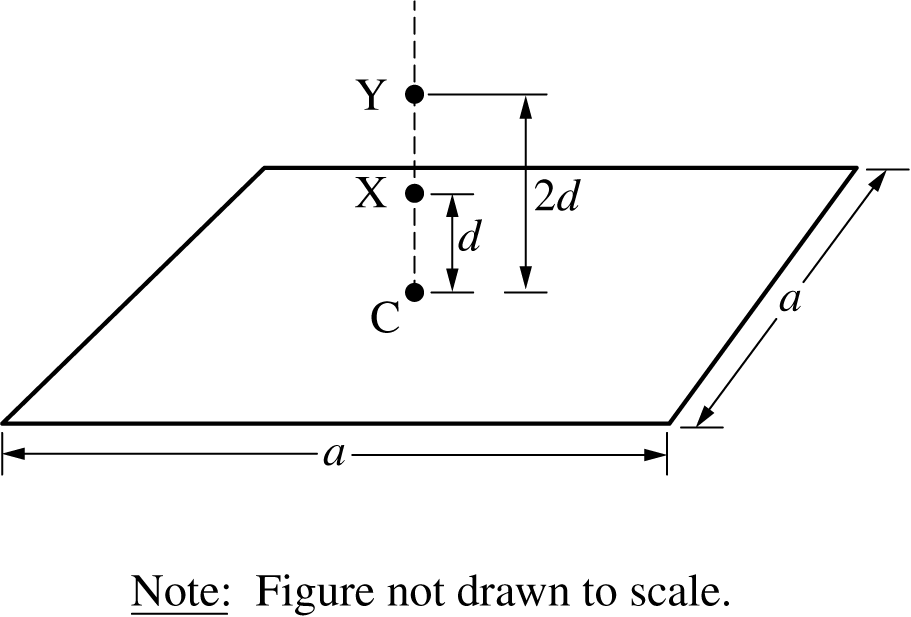
\includegraphics[scale=0.3]{images/img-002-000.png}
\end{center}

The figure above shows a thin, square, nonconducting sheet of positive charge uniformly distributed over its area. The length of each side of the sheet is $a$. Point $\mathrm{C}$ is at the center of the sheet. Point $\mathrm{X}$ is a distance $d$ above the center of the sheet, and point $\mathrm{Y}$ is a distance $2d$ above the center of the sheet. Assume $a \gg d$. The effect of gravity is negligible.

\begin{questions}
\setcounter{question}{0}

% Multiple Choice Question 1
\question
If the magnitude of the electric field at point $X$ is $E$, what is the magnitude of the electric field at point $\mathrm{Y}$?

\begin{oneparchoices}
    \choice $E / 4$
    \choice $E / 2$
    \choice $E$
    \choice $2E$
    \choice $4E$
\end{oneparchoices}

% Multiple Choice Question 2
\question
A positive point charge $+q$ is released from rest at point $\mathrm{X}$. If the magnitude of the electric field at point $\mathrm{X}$ is $E$, what is the kinetic energy of the charge at point $\mathrm{Y}$?

\begin{oneparchoices}
    \choice $q E d$
    \choice $\sqrt{2} q E d$
    \choice $2 q E d$
    \choice $2 \sqrt{2} q E d$
    \choice $4 q E d$
\end{oneparchoices}

\end{questions}
